\documentclass{article}
\usepackage[utf8]{inputenc}

\title{CS51 MiniML Extensions}
\author{Daniel Nguyen}
\date{May 2019}
\usepackage{graphicx}
\begin{document}


\maketitle

\section{Extensions}
The extensions that I implemented in the miniml interpreter are float/float operations, lexical evaluation, and exception raising. The interpreter has the ability to accept floats as expressions and perform binary and unary operations on them. On the other hand, the two main differences between lexical and dynamic evaluation is in function definition and function application. In dynamic evaluation, the environment of functions is determined when they are applied, but in lexical evaluation, the environment is determined at function definition. Therefore, functions evaluate to themselves and their current environment in a package termed a “closure.” The last extension that I implemented was custom exception raising and a mini implementation of “try with.” 

\section{Implementations}
\\
\subsection{Floats}

Float was implemented by first modifying the parser to accept float values. In miniml.lex, a rule was added that a series of digits followed by a dot (“.”) and other digits is a float value. Then, I added the “+.”, “-.”, and “*.” in the hashtable of symbols that the interpreter detects and mapped them to float operations. In miniml.parse.mly, I created a grammar rule of each float operation, Timesf, Plusf, and Minusf, and its corresponding binop operation. Now, the parser is able to accept different float values, so I then implemented the associated functions for floats, Timesf, Plusf, and Minusf, which simply imitates the ocaml float arithmetic operations. 
\\
To implement floats in our code, freevars, subst, and the eval functions minimally change. We specify that floats have no freevars or role in substitution in these functions, and in the evaluation functions, they merely evaluate to themselves. However, in our binary operators, we must add a case for Plusf, Minusf, and Timesf to evaluate when our parameters are floats. Plus, Minus, and Times are their own functions, while Equals and LessThan use previously defined functions. We reuse the equals and lessthan binop because they evaluate to some true or false, regardless of parameter type. The addition of functions Plusf, Minusf, and Timesf, which have the concrete syntax “+.”, “-.”, and “*.” respectively, enforce the barrier between integer and float arithmetic. This design decision may result  in a longer implementation, but it minimizes the possibility that a user mistakenly treats an integer as a float or vice versa.
\\
\subsection{Lexical Evaluation}
Lexical evaluation was implemented by changing the evaluation semantics in the case of function definition and application. Function definition evaluates to a closure of itself and the environment it is defined in. Meanwhile, function application evaluates an argument, with the environment of the closure, instead of the current environment. Since dynamic and lexical evaluation share many evaluation rules, I abstracted the dynamic programming rules to a general evaluation function and called this function in my dynamic and lexical evaluation functions. 
\\
\subsection{Exceptions}
A simple custom exception system was generated by modifying the parser to recognize the keyword “exception” and a following string in all caps as an expression type of exception. This changes our evaluation because if we reach the expression type of exception, then we raise an EvalError instead of continuing with our code. A mini implementation of the try/with tool in Ocaml was implemented with the following grammar: try (expression) with (expression). This allows the user to attempt to evaluate an expression and if any EvalError exception is raised, then it will evaluate the second expression instead. The parser was modified to recognize the try and with keywords and store their corresponding expressions in the Trywith expression type. Then, in each evaluation, I used an ocaml try/with to evaluate the first expression and in the case of an exception, evaluated the second expression. 

\section{Usage}
The following shows how to use the different extensions. Floats are an atomic data type and have similar functionality to ints and bools. They can be checked for equality to a value of the same time, summed, subtracted, compared, and defined in expressions and let statements. Meanwhile, the lexical evaluator is used in the same way as the dynamic and substitution evaluator, by typing the expressions in the miniml interpreter, but the way that these expressions are evaluated is different, based on the evaluation rules described before. In order to change to lexical evaluation, users must open the evaluation.ml file and change the value of evaluate to “eval\_l” or any of the other eval functions. Users can raise a custom exception by the following syntax: exception NAME, where the keyword NAME is the exception raised. The try/with tool is used in the miniml interpreter by the syntax: try (expression) with (expression), and the interpreter will first evaluate the first expression and evaluate the second in the event of an exception. The following indicate how to use the expresssions: 
\newline

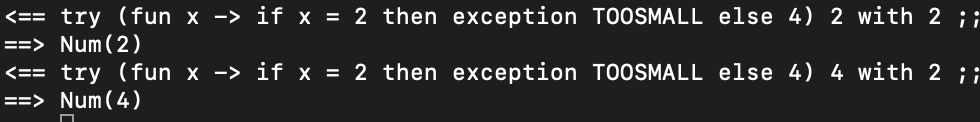
\includegraphics[scale=.8]{trywith.png}

\newline


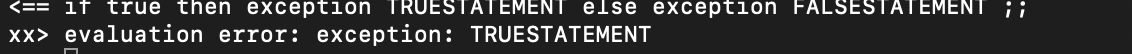
\includegraphics[scale=.8]{exception_usage.png}

\section{Challenges}
One of the biggest challenges that I encountered while implementing these extensions is understanding how the miniml\_parse and miniml\_lex tools work. I read through the resources given in the textbook, but ultimately what was most helpful was reading the code itself and recognizing patterns. I noticed that the miniml\_lex file matches user input on the standard input to a keyword. Meanwhile, the miniml\_parse file matches the keywords and their associated expressions with the expression types in expr.ml. After modifying the parser to accept certain keywords, I merely added the additional expression types to my match statements. I recognize that a large challenge in working with a less popular language is lack of resources to understand its different tools, like the parser. In this case, one of the best techniques is to experiment with code in order to understand it. 


\end{document}
